\section{Испытание системы сбора данных с использованием FLIB}\label{section:flib}

Значительная часть данных была набрана параллельно двумя системами сбора данных. Было проведено побайтное сравнение результатов распаковки обоих потоков. На массиве составляющем примерно $ 10^{7} $ сообщений расхождений не выявлено. Таким образом, продемонстрирована работоспособность концепции формирования временных интервалов и ввода данных в компьютер с использованием FLIB. Приведённые в следующих разделах результаты получены на основе данных, принятых через стандартный сетевой интерфейс с применением DAQ ПО на основе DABC~\cite{DABC}.

% FLIB
\subsubsection{FLES Interface Board}\label{sec:FLIB}

В качестве платы-интейфейса между электроникой, разрабатываемой специально для CBM, и ЭВМ стандартной архитектуры, будет выступать плата, в общем называемая платой интерфейса FLES --- FLES Interface Board, или FLIB. FLIB можно рассматривать как особый сетевой интерфейс, основной задачей которого является предоставление данных, поступающих по входным каналам, центральному процессору ЭВМ. В отличие от сетевого интерфейса Ethernet, данные поступают от разнородных плат передней электроники по разным протоколам. В качестве платформы для реализации FLIB в CBM рассматривается коммерческая PCI-E плата HTG~K-7. Архитектура FLIB показана на \figref{fig:FLIBarch}. Основные компоненты FLIB --- драйверы входных оптических портов, программируемая пользователем вентильная матрица (ППВМ, FPGA), оперативное запоминающее устройство (ОЗУ) и драйвер шины PCI-Express. 

\begin{figure}[H]
\centering
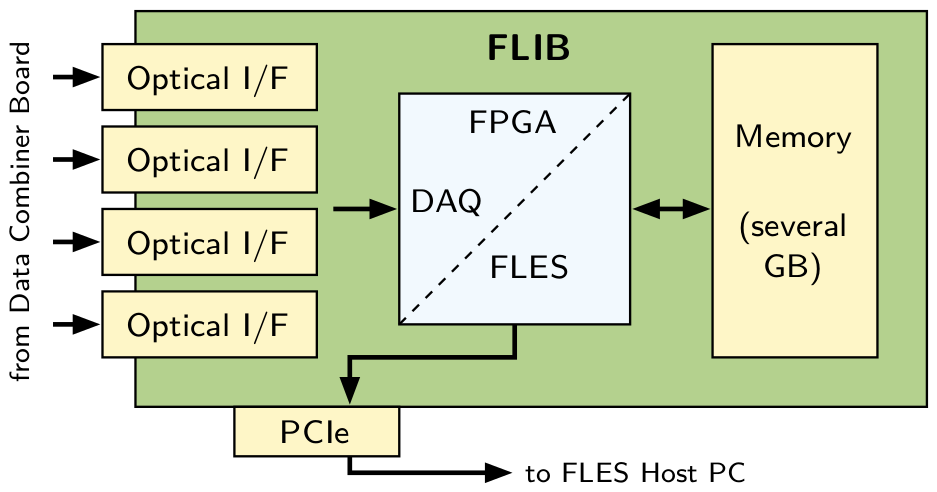
\includegraphics[width=0.6\textwidth]{pictures/FLIBarch.png}
\caption{Архитектура FLIB.}
\label{fig:FLIBarch}
\end{figure}